%%%%
% Consiglio la visione dei seguenti tutorial:
% - https://www.youtube.com/watch?v=ihxSUsJB_14
% - https://www.youtube.com/watch?v=XTFWaV55uDo
%%%%
\documentclass[12pt,a4paper,openright,twoside]{book}
\usepackage[utf8]{inputenc}

%\newcommand{\thesislang}{italian} % Italian thesis
\newcommand{\thesislang}{english} % English thesis
\usepackage{thesis-style}
% version
\newcommand{\versionmajor}{0}
\newcommand{\versionminor}{1}
\newcommand{\versionpatch}{2}
\newcommand{\version}{\versionmajor.\versionminor.\versionpatch}
\typeout{Document version: \version}

\begin{document}

\frontmatter

% ! TeX root = thesis-main.tex
\title{Title}
\author{Candidate Name Here}
\date{\today}

\newgeometry{margin=0.8in}
\begin{titlepage}
	\begin{center}
		% \vspace*{0.2cm}

		\large
		\textbf{ALMA MATER STUDIORUM -- UNIVERSITÀ DI BOLOGNA \\ CAMPUS DI CESENA}
		\\
		\noindent\hrulefill
		\vspace{0.4cm}

		\Large
		Scuola di Ingegneria e Architettura \\
		Corso di Laurea Magistrale in Ingegneria e Scienze Informatiche

		\Huge
		\vspace{4cm}
		\textbf{
			Design and implementation of a portable Framework for application decomposition and deployment in Edge-Cloud Systems
		}

		\large
		\vspace{1cm}
		Tesi di laurea in
		\\
		\textsc{Pervasive Computing}

		\vspace{5.5cm}
		\begin{minipage}[t]{0.64\textwidth}
			\begin{flushleft}
				\textit{Relatore}
				\\
				\textbf{Prof.} \textbf{Mirko Viroli}
				\\
				\vspace{0.4cm}
				\textit{Correlatore}
				\\
				\textbf{Prof.} \textbf{Danilo Pianini}
			\end{flushleft}
		\end{minipage}
		\begin{minipage}[t]{0.34\textwidth}
			\begin{flushright}
				\textit{Candidato}
				\\
				\textbf{Nicolas Farabegoli}
			\end{flushright}
		\end{minipage}\\

		\vfill
		\noindent\hrulefill
		\vspace{0.3cm}
		\Large

		Quarta Sessione di Laurea
		\\
		Anno Accademico 2022-2023
	\end{center}
\end{titlepage}
\restoregeometry

\begin{abstract}
	Max 2000 characters, strict.
\end{abstract}

\begin{dedication} % this is optional
	Optional. Max a few lines.
\end{dedication}

\begin{acknowledgements} % this is optional
	Optional. Max 1 page.
\end{acknowledgements}

%----------------------------------------------------------------------------------------
\tableofcontents
\listoffigures     % (optional) comment if empty
\lstlistoflistings % (optional) comment if empty
%----------------------------------------------------------------------------------------

\mainmatter

% Introduction --------------------------------------------------------------------------
\chapter{\introductionname}
\label{chap:introduction}
%----------------------------------------------------------------------------------------

With the Internet of Things (IoT), more and more devices are connected to the network producing a very large amount of data.
Cloud computing has been established as a technology for acquiring computational power and storage in support of various applications;
however, it is not always suitable for handling all kinds of systems' requirements: latency, security, and privacy are some of the main
concerns. This comes true especially with IoT systems since they produce lots of data and in some scenarios, they must respect real-time constraints.
For these reasons, fog computing tries to overcome the cloud's limitation by defining a computing model that sits between IoT devices and the cloud.
It allows for the collection, aggregation, and processing of data from IoT devices (or more in general edge devices) using a hierarchy of computing
power.
The combination of fog computing with the cloud can reduce data transfers and communication bottlenecks to the cloud, and can also contribute to
reduced latencies since fog computing resources are closer to the edge.

Nevertheless, realizing systems that operate in the edge-cloud continuum is an open challenge~\cite{BITTENCOURT2018134}:
the heterogeneity of the devices combined with the dynamic nature of the requirements that modern systems must have, leveraging the flexibility of
the edge-cloud continuum is found to be as strategic as it is complex.

Different approaches have been proposed to address the challenges of realizing systems that well interoperate in heterogeneous
infrastructures. Some notable methodologies and frameworks are represented by the osmotic computing paradigm~\cite{8781958}, DR-BIP and its
extensions~\cite{10.1007/978-3-030-03424-5_20,10.1007/978-3-642-30564-1_1,de2020dream}.
While the first approach is mainly oriented to distributed microservices, the latter is more focused on the orchestration of distributed
applications by dynamically adapting the system to the changing requirements basing the systems on the \emph{motif} concept.

In the CPS context, engineering systems featuring distributed intelligence in a \emph{self-organization} fashion is one of the main relevant
approaches. In this way, the global behaviour of the system is obtained by the interaction of the individual components giving robustness to the
system. The current trend of large-scale, dynamic and heterogeneous Cyber-Physical Systems requires increasingly complex and diverse
infrastructures. Remote clouds offer a seemingly supply of computing, storage, and services on demand, but this comes with the caveat of high
costs and potential latency issues, as well as data protection concerns that must align with the specific requirements of each application. Edge
computing, on the other hand, brings resources closer to users, resulting in reduced latency and increased reactivity, while simultaneously
addressing data dissemination concerns.

As stated before, such infrastructures are not easy to manage and orchestrate, complicating the engineering phase where the logic of the
system tends to be coupled with infrastructure aspects. Generally, this prevents the reusing of design elements across different scenarios by
exploiting the underlying infrastructure opportunistically.

To tackle this problem the \emph{pulverization approach} is proposed~\cite{fi12110203}: this framework brakes the system behaviour into small
computational pieces logically linked to sensors and actuators that are continuously executed and scheduled in the available infrastructure.
In this way, the system can be seamlessly mapped onto a variety of multi-layered deployment infrastructures.
It is based on a flexible logical model which can be decomposed into a set of sub-components with well-defined relationships that can be deployed and 
wired separately. The pulverization facilitates the deployment independence of a system, namely the ability to run the application with no change
on various deployments retaining its original functional semantics.
In this way, the application logic will obtain the functional goals independently of the actual deployment since the choice of the deployment 
strategy is affected typically by non-functional requirements such as latency, security, performance and cost.
This approach is formalized to provide an unambiguous specification of what constitutes pulverization by clarifying subtle aspects of the model
and state the deployment-independence property rigorously. 

The main contribution of this thesis is the development of a framework that leverages the pulverization approach to orchestrate distributed
applications in the edge-cloud continuum.
This framework aims to lay the groundwork for closing the gap between the simulation of these systems and their deployment by exploiting the
pulverizing methodology.
Although the pulverization approach originates in the context of aggregate computing, the framework aims to be generic enough to enable the
pulverization in non-aggregate systems as well.
To showcase the effectiveness of the framework, some scenarios in the context of CPS have been identified by using the framework to deploy such
systems, highlighting the potential that pulverization has as a methodology.
In particular, the framework is used in conjunction with \emph{embedded systems} to recreate a heterogeneous infrastructure where the framework
runs on.

%
\paragraph{Thesis Structure.} % Optional paragraph title
%
Accordingly, the remainder of this thesis is structured as follows.
%
\Cref{chap:background} discusses the background and related works.
%
\Cref{chap:requirements} summarize the requirements of the framework and give an overview of relevant deployment scenarios that are worth
to be considered during the validation of the framework.
%
\Cref{chap:design} presents the framework and its architectural design.
%
\Cref{chap:implementation} describes the implementation details of the framework.
%
\Cref{chap:validation} shows the validation process of the framework, including the experimental setup and the results obtained by the demos.
%
Finally, \Cref{chap:conclusions} concludes this thesis by summarizing its main contribution, with a focus on future works.
%----------------------------------------------------------------------------------------

% State of the art ----------------------------------------------------------------------
\chapter{Background}
\label{chap:background}

This chapter is organized into three sections. The first section provides an overview of the current layered and heterogeneous infrastructure
defined by the could-edge interplay. The second section describes the problem of the deployment independence of the applications by giving an
overview of the actual frameworks and methodologies. Finally, the third section describes the pulverization methodology in aggregate computing and
cyber-physical systems.

\section{Layered and heterogeneous infrastructure}
\label{sec:layered-heterogeneous-infrastructure}

Nowadays, electronic devices are capable of generating vast amounts of data, from measuring natural phenomena to human behavior.
The growth of the Internet of Things (IoT) is expected to connect virtually all objects, leading to a need to transfer, store, and process
unprecedented amounts of data.

Cloud computing has become an accessible platform for storing and processing data for a variety of applications, including IoT devices. It offers
flexibility and low initial costs, but its adoption has exposed limitations in fulfilling requirements for real-time, low-latency, and mobile
applications. Centralized cloud data centers are often physically and logically distant from the client, requiring multiple hops and causing delays
and consuming network bandwidth.

The adoption of cloud computing and the increasing ability of edge devices to generate and consume heterogeneous data requires new distributed
computing infrastructures that can handle diverse application requirements. Recent computing infrastructures that enact applications at edge devices
have improved response time and reduced bandwidth use. Fog computing has emerged as a paradigm that combines the ability to run localized
applications at the edge with the high capacity of the cloud, supporting the heterogeneous requirements of both small and large applications through
multiple layers of the computational infrastructure.

Taking advantage of the characteristics of the edge-cloud continuum enables many opportunities in the Internet of Things field, like
having systems that comply with requirements such as security, data locality, real-time computation, etc.
Nevertheless, the deployment of applications in this infrastructure is still a challenge and several approaches have been
proposed to address this issue~\cite{BITTENCOURT2018134}.

In the following section will be provided an overview of the main aspects and challenges that demonstrate the suitability of combining edge, fog,
and cloud computing for various applications used by the Internet of Things.

\subsection{Cloud Fog and Edge interplay}
\label{sec:cloud-fog-edge-interplay}

This section introduces the concepts and terminology of cloud, fog, and edge computing, discussing their main characteristics and finally, how
those paradigms can be combined to provide a more flexible and efficient solution for a wide range of applications.

\subsubsection{Cloud computing}

Over the last decade, cloud computing has become a widely adopted computing paradigm for many applications due to its dynamic characteristics such as elasticity and pay-per-use (achievable via virtualization and containerization), reaching a mature state.

Cloud providers offer on-demand computing through three main models, which are Infrastructure as a Service (IaaS), Platform as a Service (PaaS), and
Software as a Service (SaaS)~\cite{armbrust2010view}. IaaS provides users with remote access to computing power as a service, while PaaS offers a
platform for software development with necessary libraries and databases to deploy and run applications, and SaaS provides software that relies on
cloud providers' infrastructure to offload computing and/or data. The concept of Everything as a Service (XaaS) has emerged, which
includes a wide variety of cloud service levels.

Cloud services operate under a Service Level Agreement (SLA) that determines the services offered and the costs for using them. Common pricing models
include charging by time unit, amount of data transfer, and the number of requests. Cloud computing's features of elasticity, ubiquitous access, and
on-demand provisioning make it an attractive option, allowing for lower upfront investments and faster time to market, with reduced
operational costs.

\subsubsection{Fog computing}

The evolution of hardware in personal devices has increased computing capacity at the edge and the size of mobile devices has shrunk, allowing them
to run applications with reasonable complexity and quality of service (QoS). As a result, distributed computing paradigms are being utilized, where
edge devices are used to run applications and store data.

Fog computing creates a bridge between edge devices and the cloud, and introduces a hierarchy of computing capacity, with fog nodes, cloudlets, or
micro data centers located between the edge and the cloud. This hierarchy can be spread throughout the network, with nodes higher in the hierarchy
having larger computing capacity and serving more users, while nodes lower in the hierarchy are closer to the edge and have lower communication
delays.

The computing hierarchy in the fog infrastructure can offer a wider range of service levels, supporting applications that cannot be supported by
cloud computing alone. A fog infrastructure can handle applications with a variety of QoS requirements, as applications can run at a hierarchy
level that provides adequate processing capacity and meets latency requirements. Another consequence of the use of processing closer to the edge is
to reduce (aggregate) bandwidth use in the network along the path between the edge and the cloud.

\subsubsection{Edge computing}

Edge computing is a distributed computing paradigm that brings computation and data storage closer to where it is needed, reducing the distance that
data must travel and minimizing the latency for applications that require quick responses. Edge computing evolved from the growth of mobile devices
and the hardware evolution of personal devices.

The combination of higher computing capacity and edge networks enabled distributed computing paradigms that propose the utilization of edge devices
to run applications and store data. Edge computing is characterized by the use of devices such as smartphones, tablets, and IoT sensors and actuators
as sources of computational and storage resources. These devices have limited computational capacity and battery life but can support application
execution and storage capabilities.

Edge computing is expected to enable new applications in areas such as augmented reality, autonomous vehicles, and smart cities, among others, by
allowing data processing and analysis to occur closer to the data source, reducing response time and network congestion. Edge computing also enables
the collection of data from a variety of sources and the aggregation of data at the edge for further processing, analysis, and decision-making.

\paragraph*{}

Fog computing and edge computing are two related but distinct concepts in the field of distributed computing. However, they are often used
interchangeably or confused with one another, which can lead to misunderstandings and miscommunication.

One reason for the confusion is that both fog and edge computing refer to distributed computing infrastructures that process data closer to where it
is generated, such as on the edge of the network. They both aim to reduce network latency and bandwidth consumption by processing data locally rather
than sending it to a centralized cloud server.

However, the main difference between fog and edge computing lies in the level of hierarchy at which they operate. Edge computing typically refers to
processing that occurs at the outermost layer of the network, closer to end-user devices and sensors. It involves lightweight computing devices and
microservices that are often embedded in sensors, smartphones, or IoT devices.

Fog computing, on the other hand, involves a hierarchy of computing nodes that are distributed between the edge and the cloud. These nodes, also
known as fog nodes, cloudlets, or micro data centers, can be located at access points, routing devices in the network, or even at the core of the
network. The idea is to provide a distributed infrastructure that can handle data processing and analysis at different levels of the network
hierarchy while minimizing latency and bandwidth usage.

In conclusion, while fog computing and edge computing share similar goals and concepts, they are distinct in their approach and level of hierarchy.

\subsubsection{Edge-cloud continuum problems}

The edge-cloud continuum presents many challenges that must be addressed to optimize its performance. One of the primary issues is
managing the resources distributed across the continuum in a way that ensures efficient resource utilization and maintains QoS levels. This is
particularly challenging due to the heterogeneity of devices and applications that comprise the continuum, as well as the dynamic nature of the
network topology caused by device mobility and varying application requirements.

The movement of services in the Edge-Cloud infrastructure is an important consideration due to the inherent heterogeneity of the devices and
applications in the system. As edge and fog computing become more prevalent, there is a greater need for services to move between devices in the
hierarchy to optimize the use of resources and provide the required Quality of Service (QoS). However, managing the automatic adaptation of
services to different deployment locations while considering resource constraints at each level of the infrastructure is a major
challenge. Additionally, the heterogeneous network topology and frequent changes in device mobility and application requirements make it even more
complex.

% - New section ---------------------------------------------------------------

\section{Deployment independence}
\label{sec:deployment-independence}

The advantages of integrating different computing paradigms, such as cloud and edge computing, have already been acknowledged by numerous
industry and academia-based initiatives, one example is the OpenFog Consortium~\footnote{\url{https://opcfoundation.org/markets-collaboration/openfog/}}.

The cloud-edge computing integration is an open research topic since each of the two paradigms has its use cases and advantages. The cloud
computing paradigm is well suited for large-scale applications that require high computational power and storage capacity. On the other hand, edge
computing is well suited for applications that require low latency and high reliability, such as autonomous vehicles, smart cities, and industrial
automation. The integration of the two paradigms can provide a more flexible and efficient solution for a wide range of applications.
Nevertheless, the integration of the two paradigms is not trivial, and different approaches can be used to tackle this problem.

In this context, we refer to ``deployment independence'' as the ability of an application to be deployed on any computing infrastructure by
separating the business logic from deployment and infrastructure aspects. In this way, the system logic can be developed without considering the
underlying infrastructure, since they are orthogonal aspects. This approach, on the one hand, allows for better-engineered systems where aspects of
development and deployment are separated; while on the other hand, one can make the best use of the available infrastructure according to the
dynamics of the system.

The following section will review the main methodologies that are in the literature and aspire to develop systems that integrate cloud-edge
infrastructure.

\subsection{Actual frameworks and methodologies}
\label{sec:actual-frameworks-methodologies}

Many frameworks and methodologies have been proposed in the literature to handle the edge-cloud continuum problem. The different approaches
proposed vary in complexity and use cases, each trying to solve a specific problem.

Among the methodologies and frameworks worth mentioning is osmotic computing which operates in the IoT environment focusing on a three-tier
architecture by leveraging microservices that can be moved around the infrastructure and frameworks such as DR-BIP and DReAM that are based on the
concept of "motif" and interaction rules and reconfiguration rules to manage system deployment.

The following is an overview of how these two methodologies work, highlighting their main features and how they try to solve the integration problem.

\subsubsection{Osmotic computing}

Osmotic computing~\cite{8781958} utilizes a concept known as a MEL (microelement) to encompass resources, services, and data. In the realm of IoT,
MELs can be structured as a graph and relocated across various infrastructures based on factors such as cost, security, privacy, and performance.
MELs encapsulate four distinct elements: microservices that provide specific functionality, microdata representing the flow of information to and from
sensors or actuators, microcomputing that performs various computational tasks using real-time and historic data, and microactuators that control the
state of physical resources using actuators at the network edge.

Each application can be decomposed into (cooperative) subprograms to improve deployability and scalability. This decomposition, in osmotic computing,
defines several interacting MELs, which are atomic entities providing simple functionalities. A graph of MELs can include several microservices
(MS) and microdata (MD) combined to provide a specific behavior. In osmosis, containers (or virtual components) are used to deploy dynamically and
support the migration of MELs across heterogeneous systems.

In osmotic computing, the computing environment is divided into three layers: cloud data centers (L1), edge systems and micro data centers (L2), and
IoT devices (L3).
At L3, the IoT devices capture raw data from the environment at a fixed frequency or by events. The L2 layer is composed of network devices such as
routers, switches and gateways, supported by protocols like \emph{OpenFlow} or hardware that enables network components to be accessed remotely.
Finally, L1 is composed of data centers, which are large-scale computing facilities that provide a large number of computing resources and storage
capacity.
The L2 layer can collect the data coming from devices at L3 enabling the collection of raw data and performing some computations before transferring
these data to L1.

Osmotic computing is an extension of elastic resource management, in which the deployment and migration strategies of microelements (MELs) can change
over time based on changing infrastructure and application requirements. Osmotic computing automates the configuration and reconfiguration of MELs
based on factors such as quality of service, security, and runtime perturbations.

\begin{figure}[ht]
	\centering
	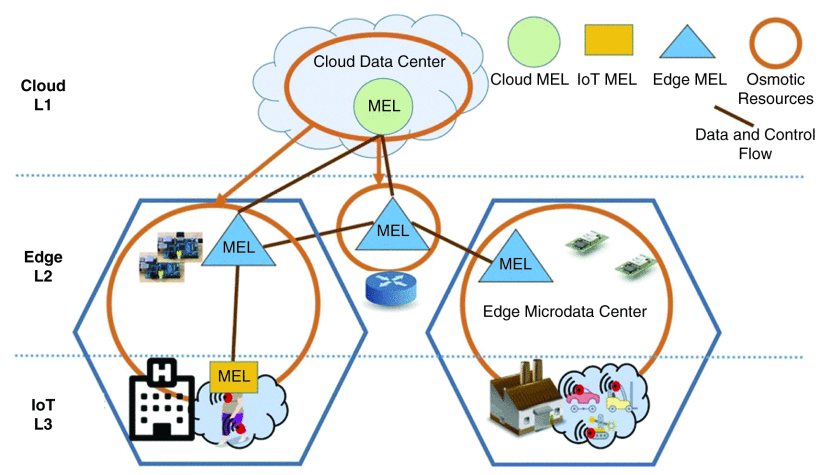
\includegraphics[width=0.8\linewidth]{figures/osmotic-architecture.png}
	\caption{Osmotic computing architecture reference. Picture taken from~\Cite{8781958}.}
	\label{fig:osmotic-computing}
\end{figure}

The purpose of an osmotic platform is to balance the needs of both the infrastructure and the applications by automatically relocating microservices
to appropriate deployment locations. This approach focuses mainly on systems that are centrally managed and coordinated.

\subsubsection{DR-BIP and DReAM framework}

The \emph{Dynamic Reconfigurable BIP} framework (DR-BIP)~\cite{10.1007/978-3-030-03424-5_20} includes three main aspects of dynamism: (I) the ability
to describe parametric system coordination for an arbitrary number of instances of component types, (II) the ability to add/delete components and
manage their interaction rules depending on dynamically changing conditions, and (III) allow services to seamlessly continue their activity on any
available device or computer (fluid architectures~\cite{taivalsaari2014liquid}).
The \emph{DR-BIP} framework is an extension of the \emph{Behavioral Interconnection Protocol} (BIP)~\cite{5719588} and
\emph{Dy-BIP} (a former extension that support dynamic interactions)~\cite{10.1007/978-3-642-30564-1_1}.

The DR-DIP framework provides support for runtime changes in the system, including component creation and removal, migration between motifs, and both
programmed and triggered reconfiguration.
The use of motifs allows components to interact with others based on their behavior and interaction rules within their new
motif, providing a flexible framework for coordination. The platform shares similarities with DReAM~\cite{de2020dream}, but the use of constraints
allows for more expressive coordination.

DR-BIP uses motifs as the basic unit for describing dynamic architectures (see~\Cref{fig:motif-concept}). Each motif includes the behavior of
components, the rules for interaction between components, and the rules for reconfiguring the motif, including adding, removing, or moving components.
Motifs are structurally organized as the deployment of component instances on a logical map.
Maps are arbitrary graph-like structures consisting of interconnected positions. Deployments relate components to positions on the map.
The definition of the motif is completed by two sets of rules: (I) the interaction rules, which define the behavior of the components and the
interaction between them, and (II) the reconfiguration rules, which define the conditions under which the motif can be reconfigured.

Systems are defined as collections of motif instances, each of which can evolve independently or in coordination with other motifs through shared
components or inter-motif reconfiguration rules. Inter-motif reconfiguration rules also allow for the creation and deletion of motif instances and
the exchange of components between motifs.

DR-BIP's behavior in a motif-based system is defined in a compositional way, where every motif has its own set of interactions determined by its
local structure. These interactions remain constant until the motif executes a reconfiguration action. In the absence of reconfigurations, the system
maintains a fixed architecture and operates like a normal BIP system. Interactions do not affect the architecture, while system and/or motif
reconfigurations change the architecture, but do not impact components, meaning running components retain their state, even though new components may
be added or removed.

\begin{figure}[ht]
	\centering
	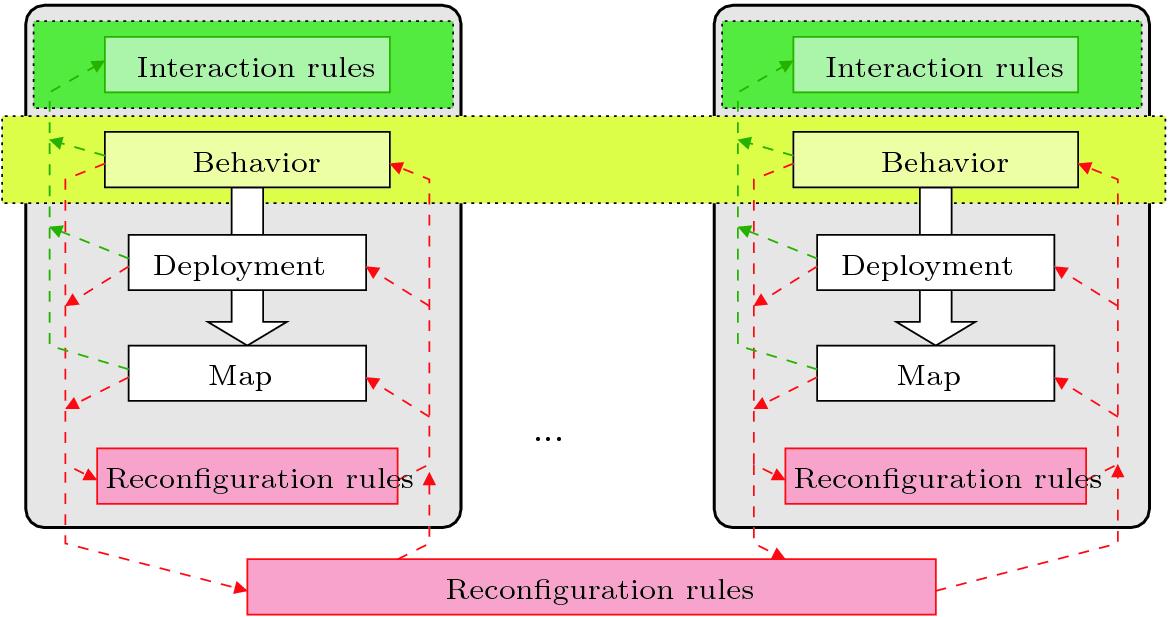
\includegraphics[width=0.8\linewidth]{figures/motif-concept.png}
	\caption{Motif-based System Concept. Picture taken from~\cite{10.1007/978-3-030-03424-5_20}.}
	\label{fig:motif-concept}
\end{figure}

% - New section ---------------------------------------------------------------

\section{Pulverization in Aggregate Computing and CPS}
\label{sec:pulverization-aggregate-computing-cps}

This section presents a brief overview of the state of the art in the field of aggregate computing and cyber-physical with a main focus on the
pulverization and which problems try to solve.

Self-organizing systems are a way of engineering distributed intelligence in which the system's global behavior and structure are achieved through
the continuous interaction of simple individual components. This approach allows for inherent adaptation to unexpected or unforeseeable situations
and has been applied in various contexts, such as human social behavior, and swarm robotics.

Artificial self-organizing systems are software-based systems that regulate their internal structures and behavior without external control, often by
mimicking the self-organization mechanisms observed in nature. Self-organizing approaches are applied to distributed cyber-physical systems (CPS),
where individual system components interact with each other based on physical proximity to collect and process information generated by distributed
sensors and use it to control the system behavior.

However, recent advances in technology have made modern CPS increasingly large-scale, heterogeneous, and dynamic, which makes it challenging to
engineer distributed intelligent systems that can be deployed in different contexts and exploit available resources opportunistically. To address
this problem, a framework based on the pulverization approach is proposed~\cite{fi12110203}, which breaks the overall system behavior into tiny
pieces of computation linked to sensors, actuators, and neighboring components. These sub-components can be deployed and wired separately, allowing
for a separation of concerns between the self-organization logic and the deployment context.

The pulverization approach can be implemented in the framework of Aggregate Computing~\cite{beal2015aggregate}, where global self-organizing behavior
can be specified declaratively by composing pure functions expressing increasingly complex distributed algorithms.
This approach allows for the design of distributed adaptive behavior for large-scale CPS that can be deployed in a deployment-independent way,
meaning that the behavioral description of the self-organization logic remains unchanged regardless of the specifics of the deployment context.

The pulverization approach was exercised simulating a CPS whose aim is to reduce the contribution of household winter heating to air pollution by
imposing a custom maximum temperature relative to the level of particulate matter (PM) in the area surrounding the household~\cite{fi12110203}.
The system implements the functionality in a self-organization fashion, where there isn't a central coordinator and the system autonomously organizes
its behaviour even in the face of disturbance.
The goal of the experiment is to show that via the pulverization approach, the system's business logic, defined once, can be reused in different
deployment schemes, preserving its functional behavior.

Another initial research effort~\cite{9599177} was made by combining the pulverization approach with the multi-tier programming
paradigm~\cite{weisenburger2020survey}.
The multi-tier programming paradigm defines a distributed architecture in a single compilation unit with a single language. Once the program is
specified, the compiler (or the runtime) is responsible for splitting the computation among different peers.
A language that supports multi-tier programming is \emph{ScalaLoci}~\cite{weisenburger2018distributed, weisenburger2020implementing}, a type-safe
multi-tier language hosted in Scala.
A ScalaLoci application is structured through \emph{peers} and \emph{ties,}where peers abstract over the locations representing the components of an
application, while the ties define the connection between peers. Only tied peers can communicate with each other.
The example provided in~\cite{9599177} shows how the pulverization approach can be fitted into the multi-tier programming paradigm, by defining
a logical node as a peer which in turn is composed of a set of peers representing the pulverized device.
Moreover, the example shows the conjunction of ScaFi, a Scala internal DSL that can run on the JVM or in the browser and ScalaLoci showing
how this could be the foundation stone of a unified framework living in the Scala ecosystem.
Finally, the example shows how different deployment schemes can be defined by changing the ties between peers by preserving the functional behaviour
of the system.

%----------------------------------------------------------------------------------------

% Design --------------------------------------------------------------------------------
\chapter{Design} % possible chapter for Projects
\label{chap:design}

This chapter describes the design choices and the overall architecture of the framework. \todo{Expand the introduction}

\section{Framework requirements}
\label{sec:framework-requirements}
\todo{Write the section about the project's requirements}

\section{Architectural design}
\label{sec:arch-design}

The framework is articulated in modules: each module takes into account a specific aspect of the pulverization.
The modularity of the framework enables from one side, the possibility to use only the needed modules, preventing the bloating of the project;
on the other side, modularity allows the customization of some implementations of the framework.

The two fundamentals modules of the pulverization framework are: \emph{core} and \emph{platform} which respectively defines the core concepts
of pulverization like the type of components and all the logic needed to run the pulverized system like defining the components reference,
loading the user-defined components and setup the communications between all of them.

The third module is \emph{rabbitmq-platform} which is highly dependent on the two modules described above and its purpose is to rely on
\textbf{RabbitMQ}\footnote{\textbf{RabbitMQ} is an open-source message-broker (or message-oriented-middleware) that originally implement
the \emph{AMQP} protocol and has since been extended with a plug-in architecture to support other protocols like \emph{MQTT}.} to enable
the communications between all the components.
This component manages all the low-level aspects related to communication like the connection to the broker, declaring queues and so on.

In~\Cref{fig:package-diagram} are represented all the framework's modules and the relationship between them.

\begin{figure}
    \centering
    \missingfigure[figwidth=\textwidth]{Package diagram showing the module relationship}
    \caption{Package diagram showing the modules that constitute the framework and their relationship.}
    \label{fig:package-diagram}
\end{figure}

The pulverization framework relies on a three-level architecture. Each level of the framework's architecture is designed to use the functionalities
of the layer above and makes accessible their functionalities to the layer below.

The described architecture takes with it the implicit ``one-way dependency'' where the layer below depends on the layer above and not vice versa.
The~\Cref{fig:framework-architecture} depicts the architecture's choice made to design and build the framework.

\begin{figure}
    \centering
    \missingfigure[figwidth=\textwidth]{Create a pyramid diagram showing the architecture of the framework emphasizing the grow-up dependency}
    \caption{Architectural diagram showing how the pulverization framework is designed.}
    \label{fig:framework-architecture}
\end{figure}

Since this is a framework, it will likely be used by several users; therefore, it is strategic to minimize the cognitive effort that the user will
have to make to use it.

For a framework to be successful and usable, it must be able to provide an incremental approach to its use,
meaning that it must provide only the abstractions necessary for its use while at the same time providing clarity in its innermost components so that
the user can understand how it works and possibly extend the framework with external modules.

The ``pyramid architecture'' used by the framework tries to apply the concept described above (\Cref{fig:pyramid-user-knowledge}):
the tip of the pyramid represents the components' abstraction defined by the pulverization and those components are used and built by the user.
Those abstraction needs to be as clear as possible from a software engineering perspective.
As you move down the pyramid, the complexity of the modules increases but the user's knowledge of them should decrease.

\begin{figure}
    \centering
    \missingfigure[figwidth=\textwidth]{pyramid architecture comparing the increase of complexity going down the pyramid and the decrease of user's knowledge going up the pyramid.}
    \caption{A correlation between the framework's complexity and the required user's knowledge to use the framework.}
    \label{fig:pyramid-user-knowledge}
\end{figure}

By designing the framework in this way, we open up different usage scenarios such as a basic use that requires only an understanding of the
basic concepts, to advanced uses that require a deep understanding of the framework but enable its complete usage and extension.

\todo{valutare se espandere qui con esempi o altro}

The sections below will describe the architectural choices made for each framework's module.

\subsection{Core module}
\label{sec:core-module}

Architecturally, the \emph{core} module is rather simple. Its simplicity is a consequence of the fact that this module is the main entry point
for the user, and the lower the complexity of this module, the faster the user can become familiar with the framework.
Moreover, a correct design of the interfaces defined in the \emph{core} module is a crucial aspect to consider to be aligned with the
pulverization concepts illustrated in the article~\cite{fi12110203}.

The pulverization represents a device as the combination of five components: \textbf{state}, \textbf{behaviour}, \textbf{communication},
\textbf{sensors} and \textbf{actuators}~\cite{fi12110203}.
The pulverization framework models the five components defined above through interfaces that the user will implement based on the specific scenario.

This module provides a DSL to generate the configuration needed for the platform to run. In particular, the DSL provides a simple, clean and handy
way to create in a declarative fashion how many logical devices should the platform manage, and how those devices are made.

\subsection{Platform module}
\label{sec:platform-module}

The platform module defines the enabling concepts for system execution like intra-component communication and provides an abstraction for
representing a remote component and how to reach it; finally, it manages all the machinery needed to run the system.

The highly distributed nature of the pulverization has forced the design phase to abstract from the actual place where components are actually
deployed; in this way, we avoid the need for the user to specify and/or manage specific aspects of deployment but can focus solely on
application logic while remaining adherent to the objectives of the pulverization, which among many want to separate aspects of 
deployment from aspects of application logic~\cite{fi12110203}.

Although the abstractions defined in this module are fundamental to the execution of the system, their understanding by the user is not essential.
Nevertheless, understanding the mechanisms defined by the platform module is important for later defining custom communicators.

As said before, communication between components is a fundamental aspect to consider; for this reason, the \emph{communicator} concept comes in.
The communicator abstracts the way how the communication between two (pulverized) components occurs, defining how two components communicate with
each other. The design of this component abstracts from the message format and the type of the involved components, effectively making the
communicator highly generic and delegating all those complexities to the platform.

Finally, the platform module provides a DSL to allow the user to instantiate the platform and then actually run the system.
The DSL allows, declaratively, to specify the components intended to be executed in that specific deployment unit, as well as indicate which
specific communicator implementation to use.

\todo{Rileggere tutta la sezione}

\subsection{Rabbitmq-platform module}
\label{sec:rabbitmq-platform-module}

This module implements a possible communicator that bases its operation on RabbitMQ. Although this module, at the time of writing, represents
the only implementation of a communicator, this does not mean that it should be the only possible solution.
Other communicators based on different technologies and infrastructures will likely be implemented in the future.

In this module, all the communication aspects that will be used for communication between components of the pulverized system are defined.
The design of the framework delegates to these types of implementations to handle low-level aspects like connections, retry on failure and so on.

While this module (or this kind of module more generally) requires a very good understanding of the concepts defined in 
section~\ref{sec:platform-module} to be implemented, it requires no cognitive effort on the part of the user to be used.

\section{Data flow in the framework}
\label{sec:framework-data-flow}

\todo{definire una sezione per valutare l'approccio asincrono dello scambio dati}

\section{Framework dynamics}
\label{sec:framework-dynamics}

The pulverization framework is designed to adapt its behaviour based on specific configurations without the need for the user to change the
business logic. This section will describe from a high-level perspective how the framework adapts its behaviour based on the configuration.

One fundamental aspect of pulverization is the ability to ``move'' the component of a device from one location to another in a transparent way.

The pulverization framework is designed to be able to take each one of the five components and set up the deployment to match the current
configuration. The framework force the user to define the components by reasoning in terms of relations between itself and the other components,
in this way, we isolate the single logic of the component and we can easily move it to another deployment unit if needed.
Moreover, by defining in this way the components, the framework can easily determine if the other component is remote or in the same deployment unit,
optimizing the communication between them.

\begin{figure}[h]
    \centering
    \missingfigure[figwidth=\textwidth]{a diagram showing how easy is to move components into another deployment unit.}
    \caption{The relation between the components of a device and the deployment unit.}
    \label{fig:framework-dynamics}
\end{figure}

This feature is fundamental to cover different scenarios and contexts where a dynamic adaptation of the system is needed. For example, considering
the case of a smart device, the system can decide to move the \emph{behaviour} from the device to a cloud service because of low batter or any other
issues, in this way the heavy computation can be offloaded to a more powerful machine so that the device can continue to run for a longer time
managing only aspects of sensing and actuation.

The \Cref{fig:dynamics-example} depicts a possible scenario where the \emph{behaviour} is moved from the device to a cloud service, depending on
the current context.
\begin{figure}
    \centering
    \missingfigure[figwidth=\textwidth]{a diagram showing the example above.}
    \caption{}
    \label{fig:dynamics-example}
\end{figure}

To achieve this dynamic feature, the framework works based on two perspectives of a single component:
\begin{itemize}
    \item \textbf{Component implemented logic} (behaviour of the component)
    \item \textbf{Component communication logic} (how the component communicates with the other components)
\end{itemize}

The first perspective is the one that the user will implement, describing and implementing the logic of the component.
The second perspective is the one that the framework will use to determine how the communication between the components should be handled.
Generally, the communication logic could be pre-defined by the framework, but the user can override it if needed.
In this way, we enable full customization of the framework giving the user the ability to define how the communication between components should
occur, or use the default implementation.

\begin{figure}[h]
    \centering
    \missingfigure[figwidth=\textwidth]{a diagram showing the two perspectives of a component.}
    \caption{}
    \label{fig:component-perspectives}
\end{figure}

The~\Cref{fig:component-perspectives} shows the two perspectives of a component, the one implemented by the user and the one used by the framework.
\todo{rileggere la sezione e vedere se ridurre il livello di dettaglio oppure introdurre nuovi concetti}

%----------------------------------------------------------------------------------------

% Implementations -----------------------------------------------------------------------
\chapter{Implementation} % possible chapter for Projects
\label{chap:implementation}


Write implementation here.

\lstinputlisting[
	float,
	language=Java,
	caption={My very first program in Java},
	label={lst:helloworld},
]{listings/HelloWorld.java}

You may need to reference listings in your thesis.
%
In this case, you are encouraged to make them \emph{floating} and reference them using labels.
%
For instance, in \Cref{lst:helloworld}, we describe a hello world program in Java.
%----------------------------------------------------------------------------------------

% Validations ---------------------------------------------------------------------------
\chapter{Validation} % possible chapter for Projects
\label{chap:validation}

Write implementation here
%----------------------------------------------------------------------------------------

% Conclusions ---------------------------------------------------------------------------
\chapter{\conclusionsname}
\label{chap:conclusions}


Write conclusions here.
%----------------------------------------------------------------------------------------

%----------------------------------------------------------------------------------------
% BIBLIOGRAPHY
%----------------------------------------------------------------------------------------

%\nocite{*} % uncomment this to show all the references in the .bib file
\bibliographystyle{plain}
\bibliography{bibliography}


\end{document}